
\documentclass[12pt]{book}
\usepackage{amsmath}
\usepackage{amsthm}
\usepackage{amstext}
\usepackage{amsopn}
\usepackage{subfigure}
\usepackage{graphicx}
\usepackage{texdraw}    %texdraw package
\usepackage{float}
\usepackage{url}

\textwidth 160mm \textheight 210mm \oddsidemargin 15pt
\evensidemargin 0pt \topmargin 0cm \headsep 0.3cm
\renewcommand\baselinestretch{1.5}

\newtheorem{theorem}{Theorem}[chapter]
\newtheorem{lemma}[theorem]{Lemma}
\newtheorem{proposition}[theorem]{Proposition}
\newtheorem{corollary}[theorem]{Corollary}

\theoremstyle{definition}
\newtheorem{definition}[theorem]{Definition}
\newtheorem{example}[theorem]{Example}
\newtheorem{xca}[theorem]{Exercise}

\theoremstyle{remark}
\newtheorem{remark}[theorem]{Remark}

\numberwithin{equation}{chapter}
\numberwithin{figure}{chapter}

\begin{document}

\frontmatter
\title{A Model for the Population\\ of the Blue Crab in the Chesapeake Bay}
\author{{\large Timothy J. Becker} \\
\\
{\small Department of Mathematics,}\\
{\small College of William and Mary,}\\
{\small Williamsburg, VA 23187-8795, USA }\\
\\
{\small Email:  tjbecker@email.wm.edu }}
\date{}
\maketitle


\pagestyle{plain}

\newcommand{\ds}{\displaystyle}
\newcommand{\ep}{\varepsilon}
\newcommand{\la}{\lambda}
\newcommand{\R}{{\mathbf R}}
\newcommand{\Rp}{{\mathbf R}^+}
\newcommand{\rn}{{\mathbf R}^n}
\newcommand{\noi}{\noindent}


\maketitle

\begin{center}
\begin{minipage}{120mm}
\begin{center}{\bf Abstract}\end{center}

We model the population of the Blue Crab in the Chesapeake Bay by
using differential equations. Blue crabs are inherently cannibalistic
of juveniles, while also in competition with juvenile blue crabs for
resources. These differential equations describe the intraguild
predation consistent in the blue crab food web, as well as the
cannibalistic nature of the blue crab. We introduce an aging and birth
rate to alter an intraguild predation model to fit the cannibalistic
nature.

\end{minipage}
\end{center}

\setcounter{page}{2}

\tableofcontents

\listoffigures


\mainmatter

\chapter{Introduction}

\section{Background on Blue Crab}

The blue crab (\textit{Callinectes Sapidus}) is an aquatic organism which plays a large role in the food chain in the Chesapeake Bay. Additionally, the blue crab is the highest grossing of any of the commercial fisheries in the Chesapeake Bay and makes up approximately one third  of the nation's catch of blue crab.  The population of the blue crab in the Chesapeake Bay has been well below its historic level, which is one of the driving factors of this study. In 2009, the adult blue crab population reached above 200 million for the first time since 1993. The population of the juveniles, however, is still well below the historic average.

The blue crab partakes in intraguild predation, which is a subset of omnivory.  Omnivory is commonly defined as predation over more than one trophic level\;\cite{HP}.  In this case, we have the blue crab, which eats both juvenile blue crabs as well as the bivalves that juvenile blue crabs eat\cite[pg. 592]{KC}.  Thus, the blue crab is a predator who eats over more than one trophic level. Omnivory such as this was thought to be quite rare in food webs, but now it has been found to be very common\cite{MH}. Even further, omnivory can act as a local stabilizer in food webs\cite{MH}. As such, it is not unexpected that the blue crab partakes in a food web that contains omnivory.

To make a model of the blue crab population with intraguild predation and cannibalism present, we must have a distinct break between juvenile and adult for the blue crab population, based on either age or size. The juvenile blue crabs are put into size classes based on their carapace width (CW). Cannibalism becomes apparent in juvenile blue crabs when they reach a size of $\ge 40$ mm CW\cite[pg. 547]{KC}. However, it is not until juveniles reach a size of $\ge 60$ mm CW that other blue crabs make up a significant portion of their diet\cite[pg. 548]{KC}. This is around the $7$th-$9$th instar, still less than one year old \cite[pg. 546]{KC}. Blue crabs specifically cannibalize intermolt juvenile blue crabs\cite[pg. 621]{KC}. As such, there is a disparity between when blue crabs become sexually mature, around $12-18$ months, and when blue crabs start to cannibalize younger blue crabs\cite{KC}. Taking all of this into account, we will conclude for the sake of this model that juveniles are up to one year in age, and adults are one year and older.

The diet for the blue crab is important to this study so as to accurately determine the population dynamics of the resource, for which the juvenile and adult blue crab will compete. Adult blue crabs consume over $99$ species, mainly mollusks ($20-40\%$ of stomach content), arthropods ($10-26\%$), chordates ($5-12\%$), and annelids ($1-7\%$), along with juvenile blue crabs\cite[pg. 592]{KC}. Juvenile blue crabs mainly feed on bivalves, crustaceans, and detritus, or plant matter\cite[pg. 548]{KC}. Figure $1.1$ shows the more detailed food web, with darker lines showing a stronger predation. From this, we can say for this study that the resource could be considered to be from the mollusk phylum, with a specific point of emphasis on bivalves.

\begin{figure}[t]
\begin{center}
       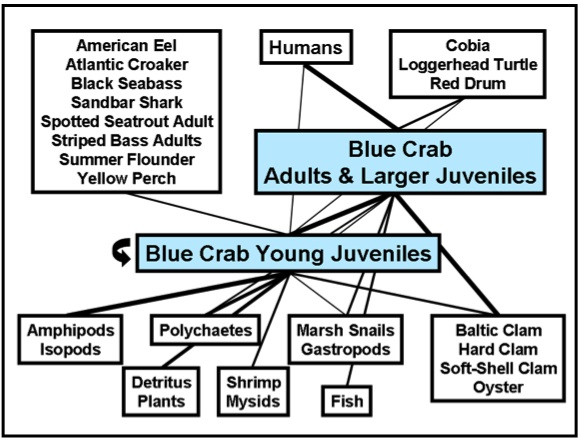
\includegraphics[width=0.8\textwidth]{foodweb.jpg}
       \caption{ Blue Crab Food Web \label{fig5}}
\end{center}
\end{figure}

\section{Basic Ecological Interactions}

There are different types of interaction that can occur between species in nature. We will focus on the two types that are prevalent to our model. The first is a Predator-Prey relationship, while the second is Competition. These two types of interaction are the foundations of complex food webs\;\cite{HP}. We do not focus on commensalism, mutualism, or amensalism here, since none are prevalent in our model\;\cite{Po}.

The Predator-Prey relationship is one that spans two different trophic levels. The predator is at one trophic level, and the prey is at a lower trophic level. The Lotka-Volterra model was one of the first models to incorporate the predator-prey relationship \;\cite{Lo,Vo}.

We have three types of functional responses that we can study as well. These describe the organism's capacity to catch, eat, and process their prey. They are the predation rate per prey as a function of the number of predators. There is the linear (Lotka-Volterra) case, as well as the more complicated Holling Type II and Holling Type III cases\;\cite{VA}.

The linear case describes a predator that eats whenever it comes into contact with prey and never becomes satiated.  As such, we have a simple term for predation $aNP$.  This term consists of a constant predation rate $a$ and then multiplied by the population of the prey, $N$, and the predator $P$.

The Holling Type II Functional Response describes a predator who eats until it is full, then processes the food, then searches for more food. Thus, we use a term that describes this behavior, namely $\ds\frac{aNP}{ahN+1}$. This term consists of the same linear case in the numerator, but also with a function in the denominator that demonstrates the capacity of the predator to become \lq\lq full\rq\rq\ based on the amount of resource available to consume\;\cite{Re}. The parameter $h$ is the handling time, which is the amount of time needed to catch, eat, and process the prey.

The Holling Type III Functional Response, which we do not use in our model, is a sigmoidal function that describes the same phenomenon of saturation of a predator at high-density levels of the prey, but also is more than just a linear relationship at low density of the prey. It is in a form $\ds \frac{aN^2P}{ahN^2+1}$. This describes the \lq\lq learning\rq\rq\ of the predator\;\cite{Re}.

\section{Review of models of Intraguild Predation and Cannibalism}


Intraguild predation is a subset of omnivory, in which two species at different trophic levels compete for prey at a lower trophic level, where a trophic level is defined as the organism's position in the food chain\;\cite{Po}.  Intraguild predation can be defined as the predation of a prey species by a predator that also preys on the resource of the prey\cite{HP}. Thus, both the predator and the prey are competitors for the resource in question, which adds a new dimension into the food web. The act of predation by the predator on the prey reduces the potential for competition for the resource\cite{Po}. Intraguild predation can also promote alternative stable states, depending on the situation\cite{Po}. Systems containing intraguild predation can produce a variety of these alternative states, as well as behaviors\;\cite{HP}.

One of the earliest models of intraguild predation was done by Holt and Polis\;\cite{HP}, and their model is in the following form:

\begin{equation}\label{11}
    \begin{split}
     \frac{dR}{dt}&=R[\phi(R)-a(R,N,P)N-a'(R,N,P)P],     \\
     \frac{dN}{dt}&=N[ba(R,N,P)R-\alpha(R,N,P)P-m],     \\
     \frac{dP}{dt}&=P[b'a'(R,N,P)R+\beta\alpha(R,N,P)N-m'],
    \end{split}
\end{equation}
where $R$ is the resource, $N$ is the intraguild prey, and $P$ is the intraguild predator\;\cite{HP}.  The resource growth rate per capita is $\phi(R)$, while $b,b'$, and $\beta$ are rates of efficiency of the predation. The functions $a(R,N,P), a'(R,N,P),$ and $\alpha(R,N,P)$ are the predation terms. The mortality rates are $m$ and $m'$ for the intraguild prey and predator, respectively. This model can be simplified to a standard Lotka-Volterra model with intraguild predation inserted into it. To make such a model, we set $a, a',$ and $\alpha$ as constants, as well as taking $\ds\phi(R)=1-\frac{R}{K}$, describing logistic growth\;\cite{HP}. The logistic growth describes the growth of the resource, beginning exponentially, but then slowing as the saturation begins, until stopping completely at a carrying capacity, $K$. We will use logistic growth for the resource in our model in Chapter 2. The simplified model is as follows:

\begin{equation}\label{22}
\begin{split}
\ds\frac{dR}{dt}&=R\left[r(1-\frac{R}{K})-aN-a'P\right], \\
\ds\frac{dN}{dt}&=N(abR-m-\alpha P), \\
\ds\frac{dP}{dt}&=P(b'a'R+\beta\alpha N-m').
\end{split}
\end{equation}

 We can also let $a,a',$ and $\alpha$ be set as Holling Type II functional responses. One of the newest models of intraguild predation is that of Verdy and Amarasekere, which uses Holling Type II functional responses \cite{VA}. This model has built upon Holt and Polis' previous model. Verdy and Amarasekere's intraguild predation model is as follows\cite{VA}:
\begin{equation}\label{3}
    \begin{split}
     \frac{dR}{dt}&=S(R)+I-E(R)-\frac{aR}{x_1}N-\frac{a'R}{x_2}P,    \\
      \frac{dN}{dt}&=\frac{baR}{x_1}N-\frac{\alpha N}{x_2}P-mN,   \\
      \frac{dP}{dt}&=\frac{b'a'R}{x_2}P+\frac{\beta \alpha N}{x_2}P-m'P,
    \end{split}
\end{equation}
where
\begin{equation*}
    x_1=ahR+1, \;\; \text{ and } \;\; x_2=a'h'R+\alpha \eta N +1;
\end{equation*}
and
\begin{equation*}
S(R)=rR\left(1-\frac{R}{K}\right), \;\; I=\rho \chi \;\; \text{and} \;\; E(R)=\tilde \rho R.
\end{equation*}
Here $R$ is the resource, $N$ is the prey, and $P$ is the predator.  The resource modeled from the logistic growth ($S(R)$), immigration ($I$), emigration ($E(R)$), and interaction between the resource and both the prey and the predator.  The rate of consumption of the resource by the prey is $a$, with a handling time $h$, and $b$ is the efficiency\;\cite{VA}.  In the same manner, $a'$ is the rate of consumption of the resource by the predator, with handling time $h'$ and efficiency $b'$, and $\alpha$ is the rate of consumption of the prey by the predator, with handling time $\eta$ and efficiency $\beta$\;\cite{VA}.  The rates of supply and loss for the resource are $\rho$ and $\tilde \rho$, and $\chi$ is the input resource concentration\;\cite{VA}. The maximum growth rate per capita is $r$, while $K$ is the carrying capacity\;\cite{VA}.  The rate of mortality of the prey is $m$ and $m'$ is the rate of mortality of the predator\;\cite{VA}.

In accordance with intraguild predation, the blue crab is inherently cannibalistic\cite{KC}(pg. 620). Thus, in terms of intraguild predation, the predator is the blue crab adult, while the prey is the blue crab juvenile. Cannibalism can be a regulator of population density and an equilibrator, while it can also result in oscillations in the population density, depending on the situations within which the cannibalism is inherent\cite{Cu}. Cannibalism can, additionally, help a population survive. The lifeboat strategy declares that what the species gains from cannibalism in times of scarcity in other resources can keep a species from going extinct when it would otherwise\cite{Cu}. Cannibalism has inherently negative and positive feedbacks which lead to many different steady states and hysteresis effects, which is a system that has \lq\lq memory\rq\rq\cite{Cu}.

\section{Summary of Results}

We will construct a model based on the intraguild predation model of Verdy and Amarasekere discussed in Section $1.3$. Our model describes the intraguild predation within the blue crab food web as well as the cannibalism that takes place on juvenile blue crabs by adult blue crabs.  Analysis shows that we have a trivial and semi-trivial equilibrium, as well as a stable co-existence equilibrium.  Bifurcation analysis shows that the blue crab model demonstrates the possibility of bistability in the system. As a caveat, we recognize that our parameter estimates are good, but not exact, and we believe that this contributes to results such as the stability of the unphysical equilibrium that was found.

\chapter{Mathematical Model}



\section{Model Setup}

We build our model based on Verdy and Amarasekere's model in Equation \ref{3}. Firstly, however, we are modeling our populations in biomass, as opposed to numbers of invididuals. We can start thinking of the predator as the cannibalistic adult, and the prey as the juvenile, as well as bivalves for the resource\;\cite{KC}. We introduce an aging term, $eN$ into the intraguild predation model, to give this model some semblance of a model with both intraguild predation and cannibalism. We introduced a Beverton-Holt birth term into the differential equation for our juveniles, which depends on the population of the adults.  This is because reproduction by the predator will increase the population of the prey, not of the predator itself. This birth term is the only increase in the model due to reproduction. Every other positive term is growth of biomass for the species, due to predation or aging. Additionally, we removed the reproduction term for the juvenile based on predation of the bivalves because the juveniles are unable to reproduce. We also assume the immigration and emigration $I=E(R)=0$ as the population in the bay is essentially closed to the outside. Additionally, we substitute in for $x_1, x_2,$ and $S(R)$ from the definitions of these parameters\;\cite{VA}. We also replace $\alpha$ with $a''$ and $\eta$ with $h''$. So, we have:

\begin{equation}\label{1}
\begin{split}
\frac{dR}{dt}&=rR\left(1-\frac{R}{k}\right)-\frac{aRN}{ahR+1}-\frac{a'RP}{a'h'R+a''h''N+1},  \\
\frac{dN}{dt}&=\frac{nP}{1+n'P}+\frac{baRN}{ahR+1}-eN-mN-\frac{a''NP}{a'h'R+a''h''N+1}, \\
\frac{dP}{dt}&=eN+\frac{b'a'RP}{a'h'R+a''h''N+1}+\frac{b''a''NP}{a'h'R+a''h''N+1}-m'P-fP,
\end{split}
\end{equation}

Thus, we have an intraguild predation model that includes the population of the juvenile depending on the birth rate of the adult and both the adult and juvenile depend on the aging rate of the juvenile.  Tables $\ref{tab1}$ and $\ref{tab2}$ describe the specific parameters and their values, so here we will describe what each term demonstrates. The equation for the resource $R(t)$ consists of the logistic term is $\ds rR\left(1-\frac{R}{K}\right),$ the term describing consumption of the resource by the juvenile is $\ds\frac{aRN}{ahR+1},$ and the term describing consumption of the resource by the cannibalistic adults is $\ds\frac{a'RP}{a'h'R+a''h''N+1}$. Both food sources are described in the denominator here to show that if $R$ goes to infinity, then this predation becomes linear in predator density, due to the amount of resource available. If $N$ goes to infinity, however, consumption of resource by adults will go to $0$ due to the increase in predation on the prey.

Similarly, we can study the equation for the juvenile population $N(t)$. The equation for the juveniles consists of the Beverton-Holt birth term is $\ds\frac{nP}{1+n'P}$.  The term describing consumption of the resource by the prey is $\ds\frac{b'a'RP}{a'h'R+a''h''N+1},$ and the term describing the aging rate of juveniles into adults is $eN$.  Lastly, we have the term for intrinsic mortality rate of juveniles as $mN$, and the term representing the predation of the juvenile by the cannibalistic adult is $\ds\frac{a''NP}{a'h'R+a''h''N+1}$. This contains both food sources in the denominator as well, for the same reasons as the adult predation on the resource.

The equation for the cannibalistic adults $P(t)$ also includes the term representing the aging of juveniles into adults: $eN$, except it is positive here. The term for the consumption of the bivalves by the adults is $\ds\frac{b'a'RP}{a'h'R+a''h''N+1}$, and the cannibalistic term for the consumption of the juveniles is $\ds\frac{b''a''NP}{a'h'R+a''h''N+1}$. Lastly, we define the losses from intrinsic mortality as $m'P$ and from harvesting as $fP$.

The flow diagram in Fig. \ref{fig1} describes graphically the interactions between the bivalves, juvenile blue crabs, and adult blue crabs. In the diagram, $G_R$ is the growth of the resource, $C_{NR}$, $C_{PR}$ and $C_{PN}$ are the consumption of resource by the juvenile, the adult, and the consumption of the juvenile by the adult respectively, $D_N$ and $D_P$ are the death of the  juvenile and adult, $M_N$ and $B_P$ are the aging and new birth, respectively, between the  juvenile and adult, and $H_P$ is the harvesting of the adult. Each of $M_N$, $C_{NR}$, $C_{PR}$ and $C_{PN}$ represent two terms (gain and loss) in the system of equations, and each of other arrows represents one term.





\section{Parameter Estimates}

We  define our time in years and our population of organisms in kilograms of biomass per square meter in the Chesapeake Bay.

\begin{table}[H]
\centering
\begin{tabular}{|c|c|c|c|}
  \hline
  \textit{Variables} & \textit{Meaning} &\textit{Dimension} & \textit{Units} \\
  \hline
  $t$ & Time & $T$ & years \\
  \hline
  $R(t)$ & Bivalves & $A$ & kg biomass/$m^2$\\
  \hline
  $N(t)$ & Juvenile Blue Crabs & $B$ & kg biomass/$m^2$ \\
  \hline
  $P(t)$ & Adult Blue Crabs & $B$ & kg biomass/$m^2$ \\
  \hline
\end{tabular}
\caption{Model variables in \eqref{1}. Dimension A is kg of resource biomass per square meter, Dimension B is kg of blue crab biomass per square meter}\label{tab1}
\end{table}

We find the predation rates of the adult blue crab in Eggleston $\cite[Table IV]{De}$, using the values for $a'$ in their paper and converting to our model. From here, we then scale our new value for our own $a'$ using the metabolic scaling rate to find the predation rate of the juvenile blue crab. We assume that predation rate is proportional to metabolic rate, so we used the allometric scaling model $\cite{BJ}$:
\begin{equation}
\ds Y=Y_0M^{3/4},
\end{equation}
for $M$ being the mass of the organism, $Y$  a dependent variable, which we take as metabolic rate, and $Y_0$ as an unknown constant of proportionality. The handling rates, $h$, $h'$, and $h''$ are determined using $T_h\;\cite[Table IV]{De}$.

For the mortality rate of the adult, $m'$, as well as the mortality due to fishing, $f$, we use the Stock Assessment of the Blue Crab in the Chesapeake Bay from 2011 $\cite{St}$. The resource growth rate, $r$, the carrying capacity, $k$, and the juvenile mortality rate, $m$, come from conversation with the researchers at the Virginia Institute of Marine Science $\cite{RM}$.

All the parameters are summarized in Table \ref{tab2}.

\begin{table}[H]
\centering
\begin{tabular}{|c|c|c|c|c|}
  \hline
  \textit{} & \textit{Meaning} & \textit{Dimension} & \textit{Value} & \textit{Source} \\
  \hline
  $r$ & Resource Growth Rate & $T^{-1}$ & 0.5 & \cite{RM} \\
  \hline
  $k$ & Carrying Capacity & $A$ & 0.2 & \cite{RM}  \\
  \hline
  $a$ & Rate of Consumption of the Resource by the Juveniles & $T^{-1}B^{-1}$ & 0.43 & \cite{De} \\
  \hline
  $h$ & Handling Time of the Juveniles for Resource Consumption & $TBA^{-1}$ & 0.1 & \cite{De} \\
  \hline
  $a'$ & Rate of Consumption of the Resource by the Adults & $T^{-1}B^{-1}$ & 1.44 & \cite{De} \\
  \hline
  $h'$ & Handling Time of the Adults for Resource Consumption & $TBA^{-1}$ & 0.1&
 \cite{De} \\
  \hline
  $a''$ & Rate of Consumption of the Juveniles by the Adults & $T^{-1}B^{-1}$ & 1.44 & \cite{De}  \\
  \hline
  $h''$ & Handling Time of the Adults for Juvenile Consumption & $T$ & 0.1& \cite{De} \\
  \hline
  $m$ & Natural Mortality Rate of the Juveniles & $T^{-1}$ & $1.5$&\cite{RM} \\
  \hline
  $e$ & Aging Rate of the Juveniles & $T^{-1}$ & $1$& \cite{RM} \\
  \hline
  $b$ & Rate of Efficiency of Resource Consumption by Juveniles & $BA^{-1}$ & $0.1$& \cite{De}\\
  \hline
  $b'$ & Rate of Efficiency of Resource Consumption by Adults & $BA^{-1}$ & $0.1$&\cite{De} \\
  \hline
  $b''$ & Rate of Efficiency of Juvenile Consumption by Adults & $1$ & $0.1$&\cite{De}\\
  \hline
  $m'$ & Natural Mortality Rate of the Adults & $T^{-1}$ & $0.9$& \cite{St}\\
  \hline
  $f$ & Fishing Mortality & $T^{-1}$ & 0.7& \cite{St} \\
  \hline
  $n$ & Proliferation Rate  & $T^{-1}$ & 1& \cite{RM}  \\
  \hline
  $n'$ & Saturation Rate & $B^{-1}$ & 1& \cite{RM}  \\
  \hline
\end{tabular}
\caption{Original Parameters in \eqref{1}}\label{tab2}
\end{table}
\vfill\pagebreak

\section{Non-dimensionalization}

We use the following change of parameters to non-dimensionalize the system:

\begin{equation}
\begin{split}
\ds s=rt, \;\; U=ahR, \;\; V=\frac{N}{b'k}, \;\; W=\frac{P}{khr}.
\end{split}
\end{equation}

Our new dimensionless  model is as follows:

\begin{equation}\label{model1}
\begin{split}
\frac{dU}{ds}&=U\left(1-\frac{U}{\kappa}\right)-\frac{\gamma_1UV}{U+1}-\frac{\la_1UW}{\theta U+\delta\psi V+1}, \\
\frac{dV}{ds}&=\frac{\nu_1W}{1+\nu_2W}+\frac{\gamma_2UV}{U+1}-\mu_1V-\frac{\delta VW}{\theta U+\delta\psi V+1}, \\
\frac{dW}{ds}&=\epsilon V-\mu_2W+\frac{\gamma_3UW+\delta \gamma_4 VW}{\theta U+\delta\psi V+1},
\end{split}
\end{equation}
where the new dimensionless parameters are:
\begin{equation}\label{con}
\begin{split}
&\kappa=ahk, \;\; \gamma_1=\frac{ab'k}{r}, \;\; \la_1=a'hk, \;\; \theta=\frac{a'h'}{ah}, \\
&\psi=\frac{h''b'}{h}, \;\; \nu_1=\frac{nh}{b}, \;\; \nu_2=n'khr, \;\; \gamma_2=\frac{b}{hr}, \;\; \delta=a''hk,\\
& \mu_1=\frac{m+e}{r},  \;\; \epsilon=\frac{eb'}{hr^2}, \;\; \gamma_3=\frac{a'b'}{ahr}, \;\; \mu_2=\frac{m'+f}{r}, \;\;
\gamma_4=\frac{b'b''}{hr}.
\end{split}
\end{equation}



The majority of the new parameters are rescaling of the old parameters, although we do have $r$ becoming $1$ and $m_2$ and $f$ being combined into $\mu_2$. All the new parameters in \eqref{model1} are summarized in Table \ref{tab3}, and the parameter values are converted from Table \ref{tab2} and \eqref{con}.
In the following chapters, we will analyze this dimensionless model \eqref{model1}.



\begin{table}[h]
\centering
\begin{tabular}{|c|c|c|}
  \hline
  \textit{} & \textit{Meaning} & \textit{Value} \\
  \hline
  $\kappa$ & Carrying Capacity  & 0.0086 \\
  \hline
  $\gamma_1$ & Rate of Consumption of the Resource by the Juveniles  & 0.0172 \\
  \hline
  $\gamma_2$ & Rate of Efficiency of Resource Consumption by Juveniles & 2 \\
  \hline
  $\gamma_3$ & Rate of Efficiency of Resource Consumption by Adults & 6.6977 \\
  \hline
  $\gamma_4$ & Rate of Efficiency of Juvenile Consumption by Adults & 0.2 \\
  \hline
  $\la_1$ &Rate of Consumption of the Resource by the Adults & 0.0288 \\
  \hline
  $\theta$ & Ratio of Adult and Juvenile Predation of Resource & 3.3488 \\
  \hline
  $\psi$ & Ratio of Handling Times & 0.01 \\
  \hline
  $\nu_1$ & Proliferation Rate of Blue Crabs & 1 \\
  \hline
  $\nu_2$ & Saturation Rate of Crab Proliferation & 0.1 \\
  \hline
  $\delta$ &Rate of Consumption of the Juveniles by the Adults  & 0.0288 \\
  \hline
  $\mu_1$ & Mortality Rate of the Juveniles & 5 \\
  \hline
  $\mu_2$ & Mortality Rate of the Adults &  3.2\\
  \hline
  $\epsilon$ &Aging Rate of the Juveniles &  4\\
  \hline
\end{tabular}
\caption{New Parameters in \eqref{model1}}\label{tab3}
\end{table}

\vfill\pagebreak

\chapter{Analysis and Simulation of the Model}

In order to incorporate both Lotka-Volterra and Holling Type II functional responses, we consider a system of equations in a more general form:

\begin{equation}\label{3.1}
\begin{split}
\frac{dU}{ds}&=U\phi(U)-a_1(U)UV-a_2(U,V)UW, \\
\frac{dV}{ds}&=\frac{\nu_1W}{1+\nu_2W}+b_1a_1(U)UV-\mu_1V-b_2a_2(U,V)VW, \\
\frac{dW}{ds}&=\epsilon V-\mu_2W+b_3a_2(U,V)UW+b_4a_2(U,V)VW,
\end{split}
\end{equation}
where all parameters are the same as in Chapter 2, $\ds \phi(U)=1-\frac{U}{\kappa}$ is the logistic growth of the bivalves, and $a_1(U)$ and $a_2(U,V)$ are predation rates.

We will consider two cases. Firstly, we have the Lotka-Volterra case, in which
\begin{equation}\label{lv}
    a_1(U)=a_1=\gamma_1, \;\; \text{ and } \;\; a_2(U,V)=a_2=\la_1.
\end{equation}
Secondly, we have the Holling Type II case, where
\begin{equation}\label{holling}
    a_1(U)=\frac{\gamma_1}{U+1}, \;\; a_2(U,V)=\frac{\la_1}{\theta U+\delta\psi V+1},
\end{equation}
and additionally we have the following new parameters:
\begin{equation}\label{holling2}
\begin{split}
b_1=\frac{\gamma_2}{\gamma_1}, \;\; b_2=\frac{\delta}{\la_1}, \;\; b_3=\frac{\gamma_3}{\la_1}, \;\; b_4=b_2\gamma_4.
\end{split}
\end{equation}
With the definitions in \eqref{holling} and \eqref{holling2}, the general system \eqref{3.1} includes \eqref{model1} as a special case.





\chapter{Conclusions}

The blue crab is  important to both the Chesapeake Bay ecosystem, as well as the economy of the area. Due to this, the decrease in population levels of the crab must be addressed. This model is constructed with the purpose of helping the Virginia Institute of Marine Science in their efforts to bring the blue crab population up to historic levels. The blue crab partakes in both intraguild predation and cannibalism, so both of these aspects must be stressed in the model.

We developed our new model based on previous intraguild predation models, especially Verdy and Amarasekere's model from 2009\;\cite{VA}. We introduced one additional feedback mechanism into their model. This is our cannibalism term. Additionally, we introduce an aging term into the model to describe the growth from the juvenile class into the adult class. We used a Beverton-Holt birth term and also a linear harvesting rate of the adult blue crab. We used both a Lotka-Volterra model and a Holling Type II model to work with a simplified model as well as a model that accurately represented the functional responses of the crabs as well as the bivalves. Thus, we determined our model for the blue crab.

We analyzed the general model for biologically reasonable parameters and found that we have the trivial equilibrium $(0,0,0)$, as well as the semi-trivial equilibria $(\kappa,0,0)$ and $(0,V^*,W^*)$. Lastly, we have the coexistence equilibrium $(U^*,V^*,W^*)$. The trivial equilibrium is always unstable, while the others are stable or unstable depending on the choice of parameters. $(\kappa,0,0)$ is the extinction equilibrium, in which the juvenile and adult blue crabs go extinct and the bivalves go to the carrying capacity, $\kappa$. It is stable for a low birthing rate of blue crabs, which we defined as our bifurcation parameter. $(U^*,V^*,W^*)$ is the coexistence equilibrium, where the juvenile and adult blue crabs persist, as well as the bivalves. This equilibrium is stable after it bifurcates from the $(\kappa,0,0)$ equilibrium. Lastly, we have the extinction of resource equilibrium $(0,V^*,W^*)$, which describes the extinction of the bivalve, but the persistence of the juvenile and adult blue crab based on cannibalism. This equilibrium is stable for some biologically non-reasonable birthing rate. Mathematically, however, we do find this equilibrium.

We simulate the model using \texttt{Matlab}, specifically \texttt{ode45}. These numerical simulations demonstrated again the three stable equilibria depending on the initial parameter value for the birthing rate. Additionally, we use \texttt{Matcont} to determine the presence of bistability in both the Lotka-Volterra and Holling Type II cases, using the calculations from the bifurcation theorem.

We hope that this work will help the Virginia Institute of Marine Science researchers in their work with the blue crab in the Chesapeake Bay. Our model will help VIMS understand the dynamics of the blue crab, including but not limited to the cannibalism in the blue crab. With this knowledge, we believe that VIMS will be able to make steps forward in their own blue crab research and conservation.

In the future, we will study the parameter estimates again, as mentioned in Section $1.4$ and work to obtain more accurate estimates. This will be used to further analyze and study the model, as well as leading to new numerical simulations.


\section{Acknowledgements}
This research is supported by William and Mary Charles Center Honors Fellowship and NSF CSUMS grant. Thank you to the best three advisors I could have possibly had. Firstly, thank you to Professor Junping Shi for approaching me to work on this project and for his constant willingness to help me at any time. Thank you to Professor Rom Lipcius for everything he taught me about the blue crab and his contagious enthusiasm for the project. Lastly, thank you to Professor Leah Shaw for answering all of my questions and helping me to understand the necessary mathematical biology for the project.

\bibliographystyle{amsalpha}
\begin{thebibliography}{MM}

\bibitem{AF} Abrams, P., Fung, S. Prey presistence and abundance in systems with intraguild predation and type-2 functional responses. Jour. Theo. Biol. 264 (2010), 1033--1042.

\bibitem{AM} Amarasekare, P. Productivity, dispersal, and the coexistence of intraguild predators and prey. Jour. Theo. Biol. 243 (2006), 121--133.

\bibitem{AM2} Amarasekare, P. Trade-offs, temporal variation, and species coexistence in communities with intraguild predation. Ecology 88 (2007), 2720--2728.

\bibitem{AM3} Amarasekare, P. Coexistence of intraguild predators and prey in resouce-rich environments. Ecology 89 (2008), 2786--2797.

\bibitem{Br} Britton, N. F. \lq\lq Essential Mathematical Biology.\rq\rq\ Springer Verlag London Limited; 2003.

\bibitem{BJ} Brown, J. H. Towards a Metabolic Theory of Ecology. Ecology 85 (7), 2004, 1771--1789.

\bibitem{CR} Crandall, Michael G.;  Rabinowitz, Paul H., 1971.
 Bifurcation from simple eigenvalues.  J. Functional Analysis, {\bf 8}, 321--340.

\bibitem{Cu} Cushing, J. M. A simple model of cannibalism.  Math. Biosci.  107  (1991),  no. 1, 47--71.

\bibitem{De} Eggleston, D.B. Functional responses of blue crabs Callinectes sapidus Rathbun feeding on juvenile oysters Crassostrea virginica (Gmelin): effects of predator sex and size, and prey size. J. Exp. Mar. Biol. Ecol.,1990, Vol 143, pp. 73-90

\bibitem{Eg} Eggleston, D.B.; Lipcius, R.N.; Hines, A.H. Density-dependent predation by blue crabs upon infaunal clam species with contrasting distribution and abundance patterns. Mar. Ecol. Prog. Ser. 85 (1992), 55-68.

\bibitem{HP} Holt, R. D.; Polis, G. A. A theoretical framework for intraguild predation. Am. Nat. 149 (1997), 745--764.

\bibitem{Lo} Lotka, A.J. \lq\lq Elements of Mathematical Biology.\rq\rq Dover Publications; New York. 1956.

\bibitem{KC} Kennedy, V., Cronin L. \lq\lq The Blue Crab:  Callinectes sapidus.\rq\rq\ Maryland Sea Grant College; College Park, Maryland. 2007.

\bibitem{KL} Kleiber, M. 1932. Body size and metabolism. Hilgardia 6: 315�332.

\bibitem{MH} McCann, K., Hastings, A., Re-evaluating the omnivory, stability relationship in food webs. Proc. R. Soc. B 264 (1997), 1249-1254.

\bibitem{Po} Polis, G., Myers, C., Holt, R. The Ecology and Evolution of Intraguild Predation. Annual Review of Ecology and Semantics 20 (1989), 297-330.

\bibitem{Re} Real, Leslie A. The Kinetics of Functional Reponse. The American Naturalist 111 (1977), 289-300.

\bibitem{RM} Romuald Lipcius, Virginia Institute of Marine Science--Personal Communication

\bibitem{St} Stock Assessment of the Blue Crab in the Chesapeake Bay 2011. University of Maryland Center for Environmental Science. 2011

\bibitem{VA} Verdy, A.; Amarasekare, P. Alternative stable states in communities with intraguild predation. Jour. Theo. Biol. 262   (2010),  116--128.

\bibitem{Vo} Volterra, V. Fluctuations in the Abundance of a Species Considered Mathematically. Nature 118 (1926) 558-560.

\end{thebibliography}




\end{document}
